%%%%%%%%%%%%%%%%%%%%%%%%%%%%%%%%%%%%%%%%%
% Beamer Presentation
% LaTeX Template
% Version 1.0 (10/11/12)
%
% This template has been downloaded from:
% http://www.LaTeXTemplates.com
%
% License:
% CC BY-NC-SA 3.0 (http://creativecommons.org/licenses/by-nc-sa/3.0/)
%
%%%%%%%%%%%%%%%%%%%%%%%%%%%%%%%%%%%%%%%%%

%----------------------------------------------------------------------------------------
%	PACKAGES AND THEMES
%----------------------------------------------------------------------------------------

\documentclass{beamer}

\mode<presentation> {

% The Beamer class comes with a number of default slide themes
% which change the colors and layouts of slides. Below this is a list
% of all the themes, uncomment each in turn to see what they look like.

%\usetheme{default}
%\usetheme{AnnArbor}
%\usetheme{Antibes}
%\usetheme{Bergen}
%\usetheme{Berkeley}
%\usetheme{Berlin}
%\usetheme{Boadilla}
%\usetheme{CambridgeUS}
%\usetheme{Copenhagen}
%\usetheme{Darmstadt}
%\usetheme{Dresden}
%\usetheme{Frankfurt}
%\usetheme{Goettingen}
%\usetheme{Hannover}
%\usetheme{Ilmenau}
%\usetheme{JuanLesPins}
%\usetheme{Luebeck}
\usetheme{Madrid}
%\usetheme{Malmoe}
%\usetheme{Marburg}
%\usetheme{Montpellier}
%\usetheme{PaloAlto}
%\usetheme{Pittsburgh}
%\usetheme{Rochester}
%\usetheme{Singapore}
%\usetheme{Szeged}
%\usetheme{Warsaw}

% As well as themes, the Beamer class has a number of color themes
% for any slide theme. Uncomment each of these in turn to see how it
% changes the colors of your current slide theme.

%\usecolortheme{albatross}
%\usecolortheme{beaver}
%\usecolortheme{beetle}
%\usecolortheme{crane}
%\usecolortheme{dolphin}
%\usecolortheme{dove}
%\usecolortheme{fly}
%\usecolortheme{lily}
%\usecolortheme{orchid}
%\usecolortheme{rose}
%\usecolortheme{seagull}
%\usecolortheme{seahorse}
%\usecolortheme{whale}
%\usecolortheme{wolverine}

%\setbeamertemplate{footline} % To remove the footer line in all slides uncomment this line
%\setbeamertemplate{footline}[page number] % To replace the footer line in all slides with a simple slide count uncomment this line

%\setbeamertemplate{navigation symbols}{} % To remove the navigation symbols from the bottom of all slides uncomment this line
}

\usepackage{graphicx}
\usepackage{booktabs} 
\usepackage[T1]{fontenc}
\usepackage{lmodern}
\usepackage{textcomp}

%----------------------------------------------------------------------------------------
%	TITLE PAGE
%----------------------------------------------------------------------------------------

\title[Pursue STEM]{Pursue STEM: Getting to know the statisticians?} % The short title appears at the bottom of every slide, the full title is only on the title page

\author[Nnenna \& Tshego]{Nnenna Asidianya \& Tshego Kelesitse} % Your name
\institute[U of T] % Your institution as it will appear on the bottom of every slide, may be shorthand to save space
{
University of Toronto \\ % Your institution for the title page
\medskip
\textit{nnenna.asidianya@mail.utoronto.ca \\ tshego.kelesitse@mail.utoronto.ca} % Your email address
}
\date{February 25, 2023} % Date, can be changed to a custom date

\begin{document}

\begin{frame}
\titlepage % Print the title page as the first slide
\end{frame}

\begin{frame}
\frametitle{Outline} % Table of contents slide, comment this block out to remove it

Nnenna \& Tshego will answer the following:

\begin{enumerate}
	\item \textbf{Who} Am I?
	\item \textbf{What} do I do?
	\item \textbf{Why} did I make the decision to study statistics?
\end{enumerate}

... and then we will play a game for you to get to know us a bit better!
\end{frame}


%------------------------------------------------


\begin{frame}
\frametitle{\textbf{Who} Am I?}
\begin{itemize}
	\item My name is Nnenna Asidianya. I am a fourth year statistics PhD student in the Department of Statistical Sciences (DOSS)
\end{itemize}
	\begin{center}
	
\includegraphics[width=0.4\linewidth]{me.jpg}
	\begin{figure}[H]
	\end{figure}
\end{center}


\end{frame}

%------------------------------------------------

\begin{frame}
\frametitle{ \textbf{What} do I do?}
\textbf{Recently years has seen an increase in the use of statistical methods by scientists in various fields. I have been actively involved in the following areas:}\\
\begin{itemize}
	\item Clinical Research 
	\item Statistical Education 
	\item Methodology 
\end{itemize}
\end{frame}

%------------------------------------------------


\begin{frame}
\frametitle{\textbf{Why} did I decide to study statistics?}
\begin{itemize}
\item First year courses: Biology I \& II, Chemistry I\& II, Physics I \& II, Calculus I\& II, \textit{\textcolor{red}{Electives: Statistics I}}
\item Second year courses: Organic chemistry I, Biochemistry I \& II, \textit{\textcolor{red}{ Electives: Linear Algebra I, Ordinary Differential Equations}}
\item Realization that I preferred my electives to my course courses.  
\item I began to take more mathematics courses in my second year of my undergraduate studies. 
\end{itemize}

\end{frame}


%------------------------------------------------


\begin{frame}
\frametitle{\textbf{Who} Am I?}
\begin{itemize}
	\item My name is Tshego and I use she/her pronouns. I am a 3rd year statistics undergraduate student majoring in Statistics and Mathematics at the University of Toronto. \end{itemize}
	\begin{center}
	\includegraphics[width=0.4\linewidth]{Tshego-Headshot.jpeg}
	\begin{figure}[H]
	\end{figure}
\end{center}


\end{frame}

%------------------------------------------------

\begin{frame}
\frametitle{ \textbf{What} do I do?}
\textbf{I am an student and a Peer Mentor in the Department of Statistical Sciences:}\\
\begin{itemize}
	\item I have taken different statistics courses showing me how to collect and analyze different types of data.
	\item I work in small teams and with campus partners to create student-centered events which are offered to STA 130 students (mentees) every other month.
	\item I provide 1-on-1 support both in person and electronically to support students with specific questions and needs such as: questions regarding statistical or actuarial science, personal questions regarding the broader U of T community, navigating on-campus activities and events, adjusting to university life.
\end{itemize}
\end{frame}

%------------------------------------------------


\begin{frame}
\frametitle{\textbf{Why} did I decide to study statistics?}
\begin{center}
	
\includegraphics[width=0.4\linewidth]{why222.jpg}
	\begin{figure}[H]
	\end{figure}
\end{center}

\end{frame}


%------------------------------------------------

\begin{frame}
\frametitle{\textbf{Pursue STEM} Supervisor}
Dr. Samantha-Jo Caetano (call me "SAM")
\begin{center}
	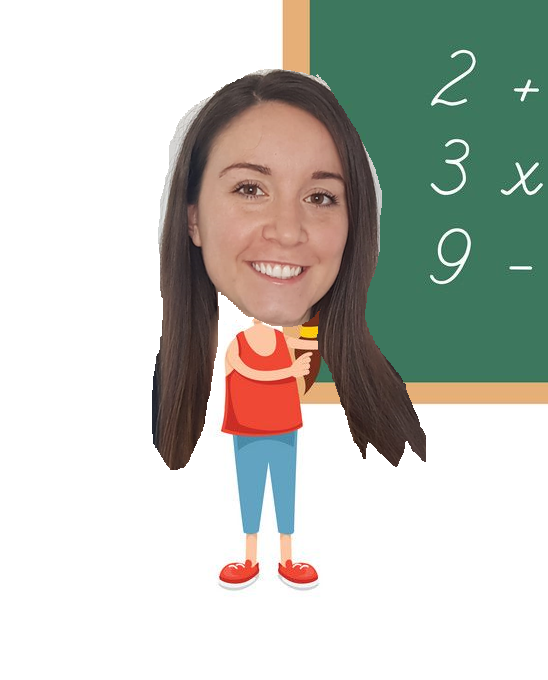
\includegraphics[width=0.3\linewidth]{Cartoon-Sam.png}
	\begin{figure}[H]
	\end{figure}
\end{center}
I am a statistics professor. If you have any questions can ask me in chat or email me at s.caetano@utoronto.ca.

\end{frame}


%------------------------------------------------


\begin{frame}
\frametitle{It's time!}

\begin{center}
Let's play "Two Truths and One Lie" to get to know us a bit better! 
\end{center}

\end{frame}


%------------------------------------------------

\begin{frame}
\frametitle{\textbf{Two Truths and One Lie:} Nnenna}

Which one is the lie about Nnenna?
\begin{itemize}
	\item My favourite gem is rhodochrosite.
	\item I have never drank coffee.
	\item My favourite colour is red.
\end{itemize}

 \vspace{0.5cm}

Go here to vote: pollev.com/sta

\end{frame}


%------------------------------------------------

\begin{frame}
\frametitle{\textbf{Two Truths and One Lie:} Tshego}

Which one is the lie about Tshego?
\begin{itemize}
	\item I can speak Persian.
	\item I watch Formula 1.
	\item I have a pet Tortoise.
\end{itemize}

 \vspace{0.5cm}

Go here to vote: pollev.com/sta

\end{frame}


%------------------------------------------------

\begin{frame}
\frametitle{\textbf{Moving Over to Content}}

Today Tshego will be leading the lesson and Nnenna will be available in chat to help with questions!  \vspace{0.5cm}

Feel free to raise your hand and unmute or type your questions in the chat!

\end{frame}


%------------------------------------------------

\end{document}